%%%%%%%%%%%%%%%%
% voda

\section{Voda}
Voda se v intru vyskytuje ve dvou formách.
V podobě vodní hladiny a v podobě tekoucí vody představující vodopády.
Vodní hladina je v intru použita pro reprezentaci moře v části s přímořskou oblastí.
Dále pak pro vizualizaci jezírek v přívodním tunelu do jeskyně a v jeskyni.
Tekoucí voda se vyskytuje až v poslední části intra - v jeskyni.
V jeskyni je několik míst, kde vyvěrá voda.
Voda stéká po stěnách, kterou zvlhčuje.

\subsection{Vodní hladina}
Vodní hladina je reprezentována prostým čtvercem.
Leskne a odráží se na ni okolí.
Odraz na vodní hladině lze vytvořit několik způsoby.

Jedním z nejjednodušších způsobů je zrcadlově převrátit scénu a vykreslit ji znovu.
Musíme si dát pozor na to, abychom vykreslovali obraz jen v oblasti vodní plochy.
Můžeme toho dosáhnou pomocí stencil testu.
Dále musíme vykreslovat jen odraz.
Nesmí se stát, aby odraz "vylézal" z vodní plochy.
Příklad takto vytvořeného odrazu je vidět na obrázku \ref{fig:reflex0}.
\begin{figure}[h]
\centering
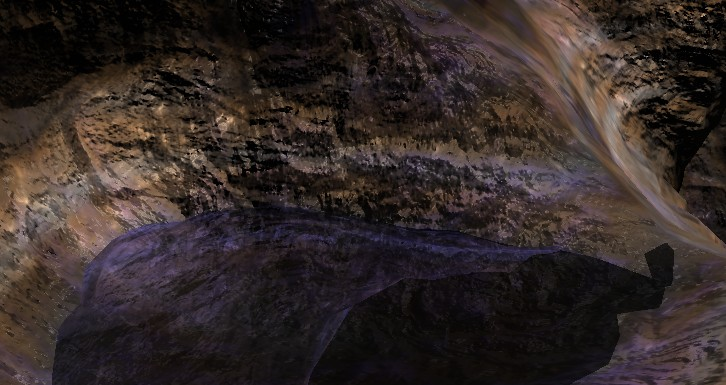
\includegraphics[width=15cm,keepaspectratio]{obr/reflex0.jpg}
\caption{Jednoduchý odraz na vodní hladině vytvořený pomocí překlopení scény.}
\label{fig:reflex0}
\end{figure}
Výhoda metody spočívá v jednoduché implementaci.
Nevýhoda je nemožnost přidat na hladinu vlnění.
Vlnění by se muselo přidávat dodatečně, jinou metodou.
Další nevýhoda je nutnost rasterizace odrazu.
Pokud se v hladině odráží celá scéna může nám výkon klesnou i na polovinu.

Jiným způsobem, jak vizualizovat odraz, je vytvořit kolem vodní plochy skybox.
Na tomto skyboxu je vykresleno okolí, které se na vodní hladině odráží.
Paprsek od kamery se podle normály vodní hladiny odrazí a směruje do určitého místa skyboxu.
Tímto získáme barvu.
Jelikož pracujeme s fragmenty a ne s celou scénou, lze poměrně snadno vytvořit na hladině vlnění.
Pokud vytvoříme skybox při inicializaci a necháme jej statický, ušetří nám to výkon.
Nemusíme scénu překreslovat pro vizualizaci odrazu.
Nevýhoda metody se skyboxem je, že se na hladině nemůže odrážet pohyblivý předmět.
Další nevýhoda spočívá v nepřesnosti odrazu.
Skybox si vytvoříme jen pro jeden konkrétní bod hladiny.
Správně bychom si jej měli vytvořit pro všechny body hladiny.
Čím vzdálenější je zkoumaný bod na hladině od bodu, kolem kterého je vytvořen skybox, tím je odraz zkreslenější.
Pokud ale hladinu vody zvlníme, nemusí být tento nedostatek patrný.
Metodu se skyboxem budeme v intru používat.

Efekt vlnění na hladině je vytvořen pomocí ovlivňování normály.
Podobně jako u bump mappingu je na hladinu namapována bump mapa.
Bump mapa nám lokálně ovlivňuje normálu, proto se povrch zdá zakřivený.
Abychom hladinu rozpohybovali, potřebovali bychom sekvenci bump map, které na sebe navazují v čase.
Sekvenci bump map si můžeme představit jako trojrozměrnou texturu.
Trojrozměrná textura obsahuje vrstvy bump map v $z$ souřadnici.
\begin{figure}[h]
\centering
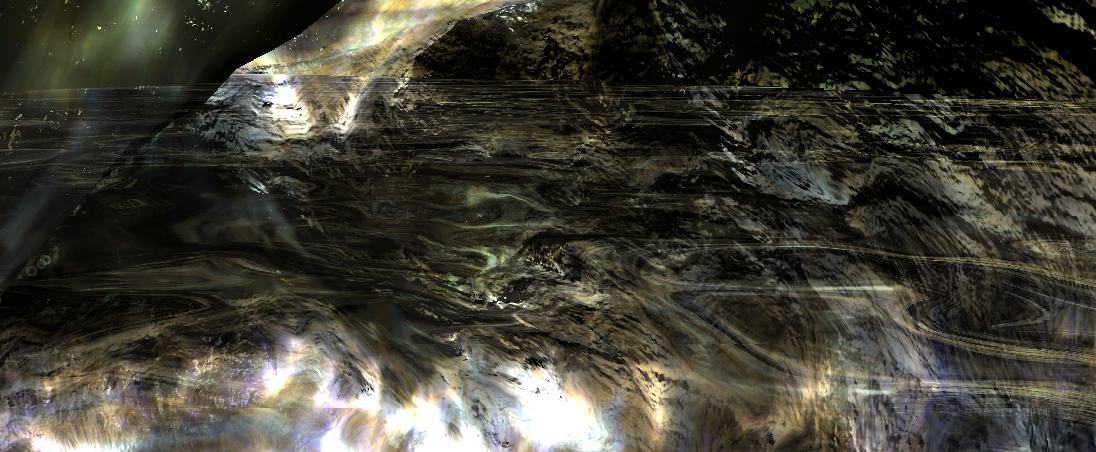
\includegraphics[width=15cm,keepaspectratio]{obr/reflex1.jpg}
\caption{Vlnění odrazu na hladině s použitím skyboxu s průhledností.}
\label{fig:reflex1}
\end{figure}


\subsection{Tekoucí voda}
Tekoucí voda je částicový systém.
Textura částic je v pravé části obrázku \ref{fig:listy}.
Jediný rozdíl je v tom, že textura není zelená ale bílá.
Tekoucí voda se vyskytuje v podobě vodopádu v poslední scéně intra.
